\section{Overall Description}\label{sec overall-desc}

\subsection{Product Perspective}
PowerEnJoy system is a simple client-server architecture based on a back-end server application and diffent front-end client applications, supported by different operating systems.

\subsubsection{User Interfaces}
Guests and users can interact with the service via the web application or the mobile application. Drivers can find other service functionalities in the car application. It is necessary to provide a common and uniform look and feel among the different hardware architectures.

All the interfaces shall be intuitive and user friendly. They should not require the reading of detailed documentation to be used.

\subsubsection{Hardware Interfaces}

All cars are provided with a dedicated embedded system connected to several plugins and a touchscreen display used for interact with the lele application.
Thanks to this embedded architecture the system will be also notified about the status of the car and its location, even if the main battery is completely discharged.

\subsubsection{Software Interfaces}

Mobile application and web application are supposed to be friendly with any device, in particular the first one must be developed for iOS and Android, and the second one will work on any operating system that support a web browser.

On the embedded system of any cars is installed a JVM that runs a Java application that provides informations to the driver and to the system.

The back-end server stores its data in a RDBMS and can run on every platform that supports the JVM. It also provides different APIs for different functions that a user, or a guest, can do through client applications. 

\subsection{Product Functions}
\begin{figure}[H]
	\centering
	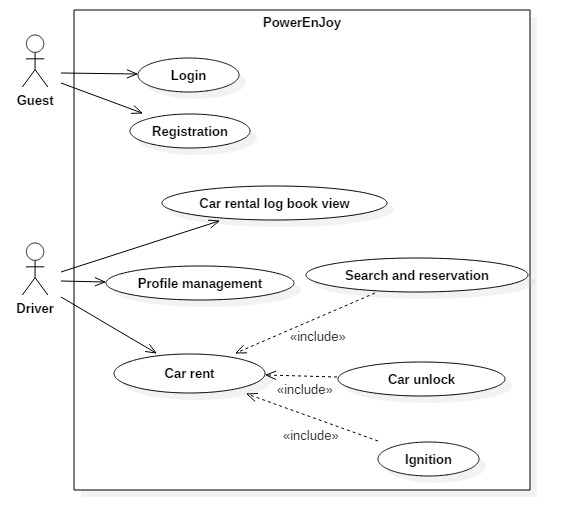
\includegraphics[width=\textwidth]{use_cases/PowerEnJoy.jpg}
	\caption{The comprehensive use-case diagram of all the functionalities implemented by the system.}
\end{figure}

\begin{figure}[H]
	\centering
	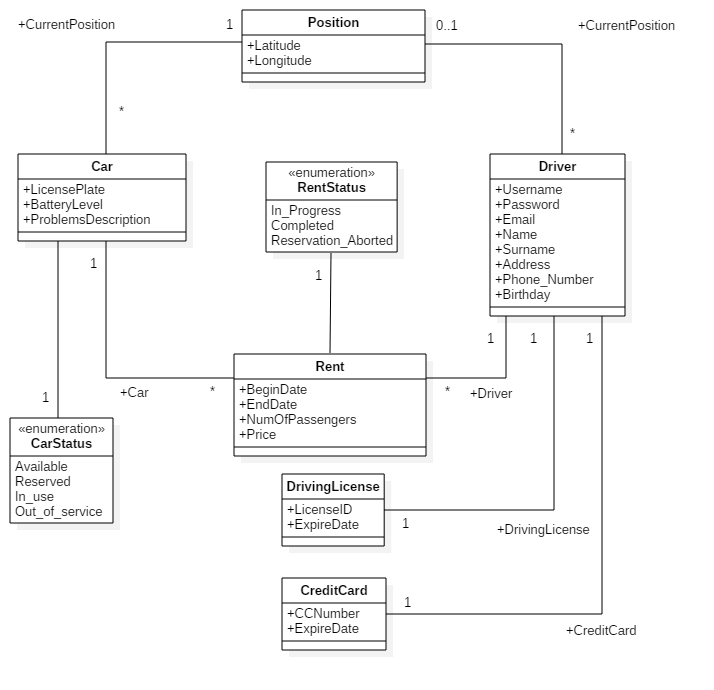
\includegraphics[width=\textwidth]{uml/PowerEnJoy.jpg}
	\caption{The comprehensive class diagram of the system.}
\end{figure}

The following lists reassume what anyone can do interacting with the system.
\begin{itemize}
	\item Guests can:
	\begin{itemize}
		\item create an account (sign up to the system)
		\item log in
	\end{itemize}
	\item Drivers can:
	\begin{itemize}
		\item edit profile informations
		\item delete their account
		\item rent a car
		\item access to the car rental log book
	\end{itemize}
\end{itemize}

\subsection{User Characteristics}

The only users of the system are drivers. Driver must provide a valid driving license and a valid payment method in order to register to the service.

It's granted that drivers have access to Internet.

\subsection{Constraints}

\subsubsection{Regulatory policies}
Any driver must follow current traffic and regulamentation laws of the area where the system is operating its car-sharing service. Driving licenses from other countries must be compatible with the laws of the country where the service is operating.

The system must ask the driver for the permission to acquire, store and process personal data and web cookies.

\subsubsection{Interfaces with other services}

PowerEnJoy ha bisogno di interfacciarsi con un servizio per risolvere tutti quei problemi che possono affliggere un veicolo o che possono generarsi durante l'utilizzo di essi.
Questi problemi possono essere:
\begin{itemize}
	\item rottura di uno o piú componenti del veicolo
	\item batteria scarica per piú del 75\%
	\item incidenti
	\item comunicazione mancante tra veicolo e sistema.
\end{itemize}
Il servizio delegato a risolvere questa tipologia di problemi, riceve tutte le segnalazioni che rientrano nei casi indicati precedentemente, e provvede a risolverli nel minor tempo possibile comunicandolo tempestivamente a PowerEnJoy.

\subsubsection{Hardware limitations}
The service requires an Internet connection fast enought to guarantee a fast response from the server and hardware architectures that can run properly the client side applications (web and mobile apps).

\subsubsection{Reliability requirements}
The system must have a minimum availability of 99\%.

\subsubsection{Parallel operations}
The system must support parallel operations from different drivers that may require access to the database.

\subsection{Domain Properties}

It suppose that the following properties hold in the analyzed domain
\begin{itemize}
	\item Once a reservation is done, it cannot be canceled by the driver.
	\item Driver's payment method and driver's driving license must be valid in order to use the rental function.
\end{itemize}

\subsection{Assumptions and Dependencies}

It assumes that:
\begin{itemize}
	\item All users have access to a stable Internet connection.
	\item Cars model is the same, so any cars will have the same number of seats.
	\item The number of cars is sufficient to satisfy the demand in each area.
	\item All the areas where the system is operating are covered by a reliable 3G/4G connection.
	\item The system is operating in an area composed by a city or agglomerated cities, of the same country, closed each other.
\end{itemize}

\subsection{Future Extensions}
The system will be implemented foreseeing the possibility of further extensions, for example:

\begin{enumerate}
	\item If a car is left at special parking areas where they can be recharged and the driver take care of pluggin the car into the power grid, the system applies a discount of 30\% on the last ride.
	\item If a car is left at more than 3 KM from the nearest power grid station or with more than 80\% of the battery empty, the system charges 30\% more on the last ride to compensate to compensate for the cost required to re-charge the car on-site.
	\item If the driver enables the money saving option, he/she can input his/her final destination and the system provides information about the station where to leave the car to get a discount. This station is determinate to ensure a uniform distribution of cars in the city and depends both on the destination of the driver and on the availability of power plugs at the selected station.
\end{enumerate}